\documentclass[12pt,a4paper]{article}
\usepackage[utf8]{inputenc}
\usepackage{amsmath}
\usepackage{amsfonts}
\usepackage{amssymb}
\usepackage{graphicx}
\usepackage{geometry}
\usepackage{float}

\geometry{margin=1in}

\title{\textbf{MSDS 7333: Case Study 5} \\ Internet Log2 Data Analysis: A Comprehensive Study of Network Traffic Classification Using Machine Learning Approaches}
\author{Tue Vu}
\date{\today}

\begin{document}

\maketitle

\newpage

\section{Introduction}

Network traffic analysis represents a critical domain in cybersecurity and network management, where understanding and classifying traffic patterns enables organizations to implement effective security policies and optimize network performance. This report presents a comprehensive analysis of Internet Log2 data, focusing on the application of machine learning techniques for network traffic classification.

The Internet Log2 dataset utilzed in this report, comprises 65,532 network traffic records collected from network monitoring systems. Each record represents a network connection session with comprehensive metadata describing the communication characteristics between source and destination endpoints.
The dataset is considered "big enough" for traditional Machine Learning models, with the regular file size of 3mb in csv format. 

This report analyses aims to achieve several key objectives:

\begin{enumerate}
    \item Conduct comprehensive exploratory data analysis to understand traffic patterns of the Internet Log2 data and data quality
    \item Develop effective preprocessing strategies for handling high-cardinality categorical variables and highly collinearity numerical features
    \item Implement and compare 2 machine learning models (in particular Support Vector Machine and Stochastic Gradient Descent) for network traffic classification
    \item Evaluate model performance and computational efficiency for large-scale deployment
    \item Provide actionable insights for network security policy implementation
\end{enumerate}

The significance of this research lies in its practical applications for network security operations, where accurate and efficient traffic classification directly impacts organizational cybersecurity posture and network performance optimization.

\section{Data}

The dataset structure encompasses 12 variables: 11 input features and one target variable. The input features are categorized into two distinct groups:

\textbf{Categorical Features (4 variables):}
\begin{itemize}
    \item \textbf{Source Port}: The originating port number of the network connection
    \item \textbf{Destination Port}: The target port number receiving the connection
    \item \textbf{NAT Source Port}: The Network Address Translation (NAT) source port
    \item \textbf{NAT Destination Port}: The NAT destination port
\end{itemize}

\textbf{Numerical Features (7 variables):}
\begin{itemize}
    \item \textbf{Bytes}: Total data volume transferred in the connection
    \item \textbf{Bytes Sent}: Volume of data transmitted from source to destination
    \item \textbf{Bytes Received}: Volume of data received from destination to source
    \item \textbf{Packets}: Total number of packets exchanged
    \item \textbf{Elapsed Time (sec)}: Duration of the connection session
    \item \textbf{pkts\_sent}: Number of packets transmitted from source
    \item \textbf{pkts\_received}: Number of packets received at source
\end{itemize}

\textbf{Target Variable:}
The \textbf{Action} variable represents the network security decision applied to each connection, categorized into four distinct classes:
\begin{itemize}
    \item \textbf{Allow}: Connections permitted through the network
    \item \textbf{Drop}: Connections silently discarded without notification
    \item \textbf{Deny}: Connections explicitly rejected with notification
    \item \textbf{Reset}: Connections terminated with reset signals
\end{itemize}

The exploratory data analysis phase provides crucial insights into data quality, feature characteristics, and underlying patterns that inform subsequent modeling decisions. This comprehensive analysis encompasses missing value assessment, categorical variable examination, numerical variable correlation analysis, and feature engineering considerations.

A critical first step in any data science project involves assessing data completeness. The Internet Log2 dataset demonstrates exceptional data quality, with zero missing values across all 12 variables. This complete dataset eliminates the need for imputation strategies and ensures that all 65,532 records contribute meaningfully to the analysis.
The absence of missing data is particularly valuable in network traffic analysis, where incomplete records could indicate data collection issues or network monitoring gaps that might bias model performance.

The distribution of the Action variable reveals significant class imbalance, a common characteristic in network security datasets, as illustrated in Figure \ref{fig:action_distribution}.

\begin{figure}[H]
    \centering
    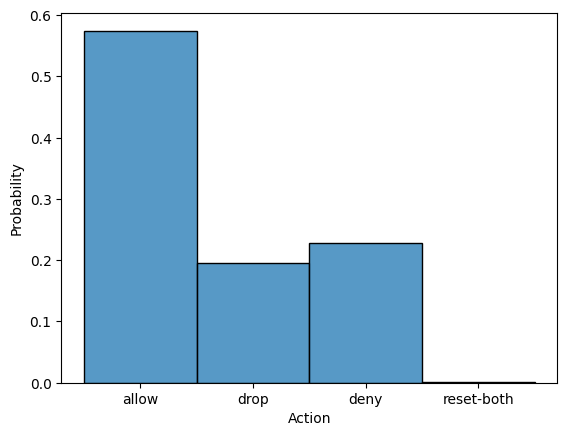
\includegraphics[width=0.8\textwidth]{figures/action_distribution.png}
    \caption{Distribution of Network Action Types showing class imbalance with Allow actions dominating approximately 60\% of all traffic, while Reset actions constitute a minimal percentage.}
    \label{fig:action_distribution}
\end{figure}

The distribution characteristics include:

\begin{itemize}
    \item \textbf{Allow}: Approximately 60\% of all traffic (dominant class)
    \item \textbf{Drop}: Substantial portion of blocked traffic
    \item \textbf{Deny}: Moderate portion of explicitly rejected connections
    \item \textbf{Reset}: Minimal representation, constituting a very small percentage
\end{itemize}

This imbalanced distribution reflects real-world network traffic patterns, where legitimate traffic typically dominates over security-blocked connections. The extreme underrepresentation of the "Reset" class presents particular challenges for model training and evaluation.

We first take a detail look into the 4 categorical features: the four port-based categorical variables exhibit dramatically different cardinality characteristics, necessitating sophisticated encoding strategies:
Table \ref{tab:cat1} tabulates the very large unique values for each port and also the unique in percentage overall the entire dataset.
We can see that both Source Port and NAT Source Port have huge amount of unique values (more than 22000 ports) whilst the 2 Destination Ports also have around 3000 unique ports.
However, in comparison, Source Ports tend to have more diverse values.

\begin{table}[H]
    \centering
    \caption{Unique values for categorical data analyses}
    \begin{tabular}{|l|r|r|r|}
    \hline
    \textbf{Feature} & \textbf{Unique Values} & \textbf{Total Records} & \textbf{Percentage Unique} \\
    \hline
    Source Port & 22,724 & 65,532 & 34.68\% \\
    \hline
    Destination Port & 3,273 & 65,532 & 4.99\% \\
    \hline
    NAT Source Port & 29,152 & 65,532 & 44.49\% \\
    \hline
    NAT Destination Port & 2,533 & 65,532 & 3.87\% \\
    \hline
    \end{tabular}
    \label{tab:cat1}
\end{table}

Detailed analysis of the top 10 most frequent ports reveals important networking patterns, as shown in Figure \ref{fig:port_distribution}.

\begin{figure}[H]
    \centering
    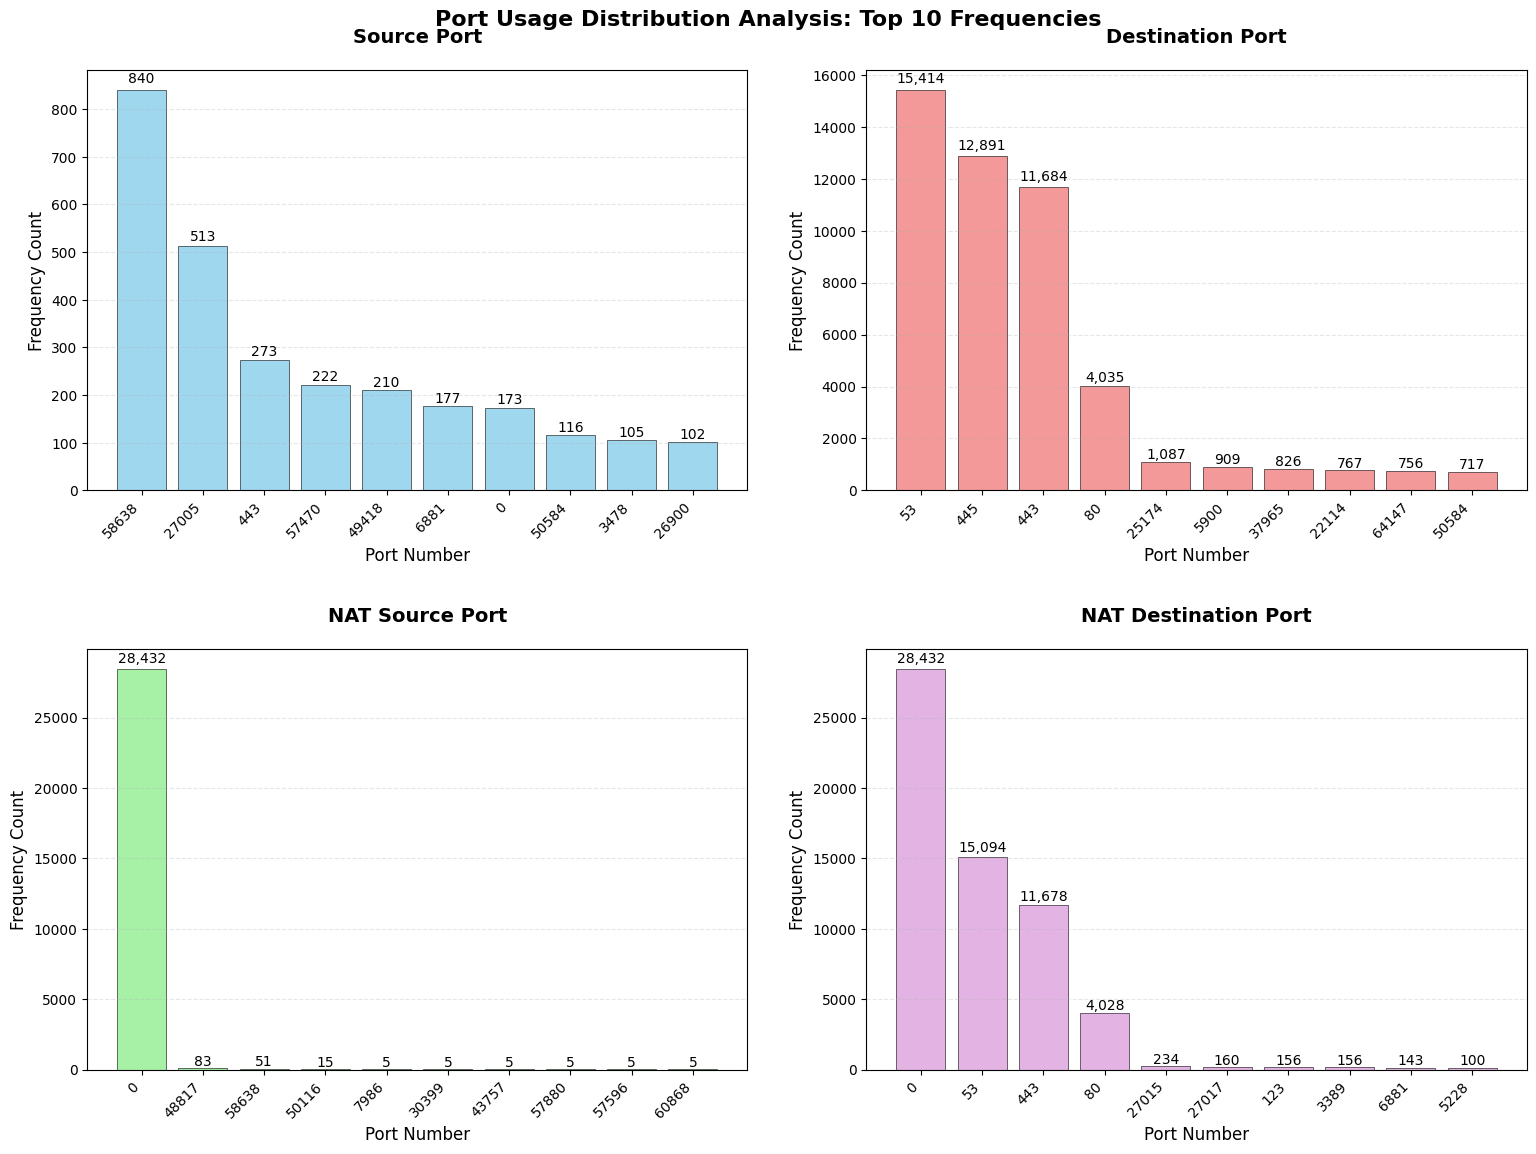
\includegraphics[width=1.0\textwidth]{figures/port_distribution.png}
    \caption{Port Usage Distribution Analysis showing the top 10 most frequent ports across all four categorical variables. Source and NAT Source ports show high-numbered ephemeral ports, while Destination ports are dominated by standard service ports (53, 443, 80).}
    \label{fig:port_distribution}
\end{figure}

\textbf{Source and NAT Source Ports:}
\begin{itemize}
    \item Common high-numbered ports in Source Port (58638, ephemeral range)
    \item Significant presence of port 0 in NAT Source Port (placeholder/invalid port indicator)
    \item Wide distribution suggesting dynamic port allocation
\end{itemize}

\textbf{Destination and NAT Destination Ports:}
\begin{itemize}
    \item Port 53: DNS traffic (highly prevalent)
    \item Port 443: HTTPS/TLS encrypted web traffic
    \item Port 80: HTTP web traffic
    \item These standard service ports dominate destination traffic
\end{itemize}

The prevalence of port 0, particularly in NAT Source Port data, indicates the presence of placeholder or invalid port assignments in the dataset. While port 0 is technically invalid (valid port range: 1-65535), its retention provides valuable information about network configuration patterns.

Given the extreme cardinality of Source Port (22,724 unique values) and NAT Source Port (29,152 unique values), traditional one-hot encoding would generate prohibitively sparse feature matrices with tens of thousands of columns. This approach would result in:

\begin{itemize}
    \item Exponential memory requirements
    \item Computational inefficiency in model training
    \item Curse of dimensionality problems
    \item Model interpretability challenges
\end{itemize}

To address these challenges, we implement a \textbf{Top-N encoding strategy} with the following methodology:

\begin{enumerate}
    \item \textbf{Frequency Analysis}: Calculate value frequencies for each categorical variable
    \item \textbf{Threshold Selection}: Retain the top 1\% most frequent values for each variable
    \item \textbf{Category Consolidation}: Group all remaining values into an "Other" category
    \item \textbf{One-Hot Encoding}: Apply standard OHE to the reduced categorical sets
\end{enumerate}

This approach balances information preservation with computational efficiency. The 1\% threshold was selected through careful consideration of:
\begin{itemize}
    \item Information retention vs. dimensionality reduction trade-off
    \item Computational constraints for model training
    \item Interpretability requirements for business stakeholders
\end{itemize}

The Top-N encoding reduces the feature space from potentially 57,682 binary features (sum of all unique categorical values) to approximately 580 features (1\% of each categorical variable plus "Other" categories), representing a 99\% dimensionality reduction while preserving the most informative categorical patterns.

Subsequently, we look at 7 numerical features with more detailed analyses using heatmap cross correlation and Variable Inflation Factor to address the collinearity issues.
The correlation matrix for numerical variables reveals critical insights into feature relationships, as visualized in Figure \ref{fig:correlation_heatmap}.

\begin{figure}[H]
    \centering
    
\includegraphics[width=0.9\textwidth]{figures/correlation_heatmap.png}
    \caption{Correlation Matrix of Numerical Variables showing strong positive correlations within and between Bytes groups and Packets groups, with Elapsed Time demonstrating relative independence from other variables.}
    \label{fig:correlation_heatmap}
\end{figure}

Key correlation insights include:

\begin{itemize}
    \item \textbf{Strong Positive Correlations}: High correlation between Bytes groups (Bytes, Bytes Sent, Bytes Received) and Packets groups (Packets, pkts\_sent, pkts\_received)
    \item \textbf{Architectural Relationships}: Bytes = Bytes Sent + Bytes Received; Packets = pkts\_sent + pkts\_received
    \item \textbf{Independence}: Elapsed Time demonstrates relative independence from other variables
\end{itemize}

Variance Inflation Factor analysis quantifies the severity of multicollinearity among numerical predictors:

\textbf{Initial VIF Analysis (All Variables):}
\begin{itemize}
    \item Bytes, Bytes Sent, Bytes Received: VIF = infinity (perfect multicollinearity)
    \item Packets, pkts\_sent, pkts\_received: VIF = infinity (perfect multicollinearity)
    \item Elapsed Time: VIF = 1.02 (acceptable)
\end{itemize}

The infinite VIF values confirm perfect linear relationships among byte and packet variables, necessitating feature selection to avoid numerical instability in model training.
Thus we suggest to remove 4 depentdent numerical features and retain only aggregated variables (Bytes, Packets, Elapsed Time). The recalculated VIF among these 3 numerical features reveal:
\begin{itemize}
    \item Bytes: VIF = 19.78
    \item Packets: VIF = 19.78
    \item Elapsed Time: VIF = 1.02
\end{itemize}

The reduced VIF values of approximately 20 for Bytes and Packets, while elevated, remain within acceptable ranges for model training. These variables capture the essential information content while eliminating perfect multicollinearity.
These 3 remaining numerical features were then standardized before merging with OHE categorical dataset.

In overall, this comprehensive preprocessing approach results in a final feature matrix with approximately 580 features with about 65000 rows of data, representing a substantial dimensionality reduction from the original high-cardinality categorical space while preserving essential information content for accurate traffic classification.
We will proceed next with Machine Learning models to classify the Action network patterns.

\section{Machine Learning Modeling}

This section presents a comprehensive comparison of Support Vector Machine (SVM) and Stochastic Gradient Descent (SGD) classifiers for network traffic classification. The analysis encompasses hyperparameter optimization, cross-validation assessment, computational efficiency evaluation, and performance comparison through multiple metrics.
The entire dataset is partitioned into training ($80\%$) and testing ($20\%$) and 5-fold cross validation where applicable.

The selection of SVM and SGD classifiers is motivated by several factors relevant to network traffic classification:

\begin{itemize}
    \item \textbf{SVM Strengths}: Excellent performance on medium-sized datasets, robust handling of high-dimensional feature spaces, and strong theoretical foundations
    \item \textbf{SGD Advantages}: Computational efficiency for large datasets, scalability to massive data volumes, and comparable performance to more complex algorithms
    \item \textbf{Linear Separability}: Initial analysis suggests that network traffic classes may be linearly separable, making linear models appropriate
    \item \textbf{Interpretability}: Both models provide insights into feature importance for security policy development
\end{itemize}

\subsection{Support Vector Machine (SVM) Analysis}

SVM performance was evaluated across multiple regularization parameter (C) values using 5-fold cross-validation and linear kernel. The comprehensive hyperparameter search examined C values spanning four orders of magnitude as tabuled in Table \ref{tab:SVMHyper}:

\begin{table}[H]
    \centering
    \caption{Regularization Hyperparameter "C" thru Cross Validation in SVM}
    \begin{tabular}{|l|r|}
    \hline
    \textbf{C Parameter} & \textbf{Mean CV Score} \\
    \hline
    0.001 & 0.9878 \\
    \hline
    0.01 & 0.9951 \\
    \hline
    0.1 & 0.9951 \\
    \hline
    1.0 & 0.9960 \\
    \hline
    10.0 & 0.9965 \\
    \hline
    100.0 & 0.9968 \\
    \hline
    1000.0 & 0.9970 \\
    \hline
    \end{tabular}
    \label{tab:SVMHyper}
\end{table}

The results demonstrate several key insights:

\begin{itemize}
    \item \textbf{Performance Plateau}: CV scores plateau above C = 0.01, suggesting optimal regularization
    \item \textbf{Marginal Improvements}: Higher C values yield diminishing returns in accuracy
    \item \textbf{Stability}: Consistent performance across the optimal range indicates robust model behavior
    \item \textbf{Linear Kernel Effectiveness}: The linear kernel achieves exceptional performance ($>99.5\%$), eliminating the need for complex polynomial or RBF kernels
\end{itemize}

SVM training on this dataset (65,532 samples × ~580 features) presents significant computational challenges:

\begin{itemize}
    \item \textbf{Quadratic Complexity}: SVM optimization scales approximately O(n²) to O(n³) with sample size
    \item \textbf{Memory Requirements}: Kernel matrix storage demands substantial memory resources
    \item \textbf{Training Time}: Very long, it easily took up to more than 5 hours for cross validation search with varying "C"
    \item \textbf{Scalability Limitations}: Performance degradation with larger datasets
\end{itemize}

Despite achieving excellent accuracy, SVM's computational demands limit its applicability for real-time network traffic classification in high-volume environments.

\subsection{Stochastic Gradient Descent (SGD) Analysis}

The SGD classifier was configured with optimization-focused parameters:

\begin{itemize}
    \item \textbf{Loss Function}: Log-loss for probabilistic output compatibility
    \item \textbf{Maximum Iterations}: 1,000 with early stopping criteria
    \item \textbf{Validation Strategy}: 10\% validation split for convergence monitoring
    \item \textbf{Convergence Tolerance}: 1e-3 for stable optimization
    \item \textbf{Early Stopping}: 5 iterations without improvement threshold
    \item \textbf{Learning rate}: is kept at constant
    \item \textbf{eta0}: the initial learning rate
\end{itemize}

SGD cross-validation results demonstrate competitive performance with superior computational efficiency (Table \ref{tab:SGDCV}):

\begin{table}[H]
    \centering
    \caption{Cross Validation and Accuracy Score for each fold for SGD}
    \begin{tabular}{|l|r|}
    \hline
    \textbf{CV Fold} & \textbf{Accuracy Score} \\
    \hline
    Fold 1 & 0.9947 \\
    \hline
    Fold 2 & 0.9947 \\
    \hline
    Fold 3 & 0.9951 \\
    \hline
    Fold 4 & 0.9950 \\
    \hline
    Fold 5 & 0.9952 \\
    \hline
    \textbf{Mean CV Score} & \textbf{0.9949} \\
    \hline
    \end{tabular}
    \label{tab:SGDCV}
\end{table}
    

\textbf{Computational Performance}: SGD cross-validation completed in 3 seconds (wall time), representing a dramatic improvement over SVM training times.

\subsection{Model Performance Comparison}

The Classification report for both models are tabulated in Table \ref{tab:SVMreport} and Table \ref{tab:SGDreport}

\begin{table}[H]
    \centering
    \caption{SVM Classification Performance}
    \begin{tabular}{|l|r|r|r|r|r|}
    \hline
    \textbf{Class} & \textbf{Precision} & \textbf{Recall} & \textbf{F1-Score} & \textbf{Support} & \textbf{AUC} \\
    \hline
    Allow & 1.00 & 1.00 & 1.00 & 7,557 & 1 \\
    \hline
    Deny & 1.00 & 0.99 & 0.99 & 2,942 & 1 \\
    \hline
    Drop & 1.00 & 1.00 & 1.00 & 2,601 & 1 \\
    \hline
    Reset-both & 0.00 & 0.00 & 0.00 & 7 & 0.98 \\
    \hline
    \end{tabular}
    \label{tab:SVMreport}
\end{table}

\begin{table}[H]
    \centering
    \caption{SGD Classification Performance}
    \begin{tabular}{|l|r|r|r|r|r|}
    \hline
    \textbf{Class} & \textbf{Precision} & \textbf{Recall} & \textbf{F1-Score} & \textbf{Support} & \textbf{AUC} \\
    \hline
    Allow & 1.00 & 1.00 & 1.00 & 7,557 & 1 \\
    \hline
    Deny & 0.99 & 1.00 & 0.99 & 2,942 & 1 \\
    \hline
    Drop & 1.00 & 1.00 & 1.00 & 2,601 & 1 \\
    \hline
    Reset-both & 0.00 & 0.00 & 0.00 & 7 & 0.98 \\
    \hline
    \end{tabular}
    \label{tab:SGDreport}
\end{table}

Both models demonstrate exceptional performance across major traffic classes:

\begin{itemize}
    \item \textbf{Perfect Classification}: Near-perfect precision and recall for Allow, Drop, and Deny classes
    \item \textbf{Class Imbalance Impact}: Reset-both class shows zero performance metrics due to extreme underrepresentation (7 samples)
    \item \textbf{Comparable Accuracy}: Both models achieve 99.5\%+ weighted average performance
    \item \textbf{Minimal Performance Difference}: SGD matches SVM performance with marginal variations
\end{itemize}

Receiver Operating Characteristic (ROC) curves provide additional performance insights through Area Under Curve (AUC) analysis, as shown in Figure \ref{fig:roc_comparison}.

\begin{figure}[H]
    \centering
    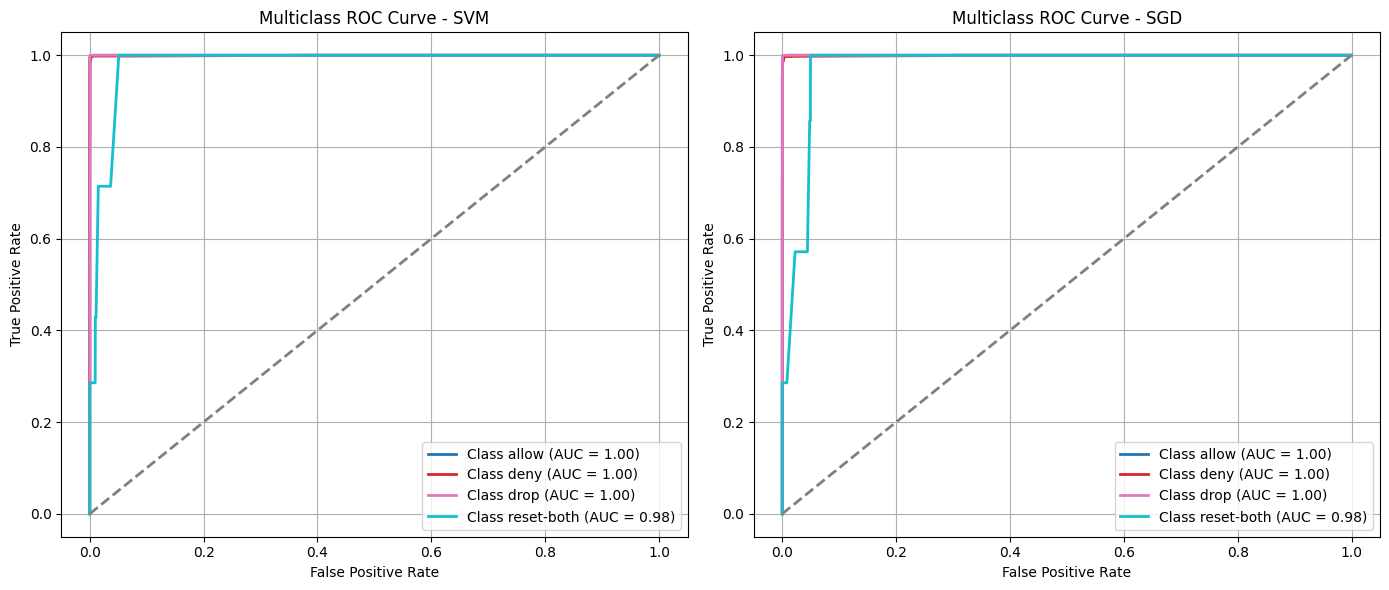
\includegraphics[width=1.0\textwidth]{figures/roc_comparison.png}
    \caption{ROC Curve Comparison between SVM and SGD classifiers showing exceptional discriminative ability (AUC ≈ 1.00) for all major traffic classes, with both models demonstrating nearly identical performance characteristics.}
    \label{fig:roc_comparison}
\end{figure}

The ROC analysis confirms exceptional discriminative ability for both models across major traffic classes, with identical performance limitations for the severely underrepresented Reset-both class.

\section{Discussions and Conclusions}

\subsection{Discussions}

This comprehensive analysis of Internet Log2 data demonstrates the successful application of machine learning techniques for network traffic classification, yielding significant insights for both methodological approaches and practical deployment considerations in cybersecurity operations.

The Internet Log2 dataset exhibited exceptional data quality with zero missing values across 65,532 records, providing a robust foundation for analysis. The preprocessing pipeline successfully addressed several critical challenges:

\begin{itemize}
    \item \textbf{High-Cardinality Management}: The Top-N encoding strategy effectively reduced dimensionality from 57,682 potential categorical features to approximately 580 features, achieving 99\% dimensionality reduction while preserving essential information content.
    \item \textbf{Multicollinearity Resolution}: VIF analysis and feature selection eliminated perfect multicollinearity among numerical variables, reducing infinite VIF values to acceptable ranges (~20) for model stability.
    \item \textbf{Feature Engineering Success}: The integration of categorical and numerical preprocessing created a balanced feature matrix suitable for machine learning algorithms.
\end{itemize}

Both SVM and SGD classifiers demonstrated exceptional performance capabilities:

\begin{itemize}
    \item \textbf{Classification Accuracy}: Both models achieved $>99.5\%$ weighted average accuracy across major traffic classes
    \item \textbf{Class-Specific Performance}: Perfect or near-perfect precision and recall for Allow, Drop, and Deny classes
    \item \textbf{ROC-AUC Excellence}: Area under curve values approaching 1.0 for all major classes
    \item \textbf{Cross-Validation Stability}: Consistent performance across 5-fold cross-validation indicates robust generalization
\end{itemize}

The analysis revealed dramatic computational differences between SVM linear kernel and SGD.
The success of linear kernels in SVM and linear SGD models provides important insights:

\begin{itemize}
    \item \textbf{Problem Characteristics}: Network traffic classification exhibits linear separability characteristics, eliminating the need for complex non-linear transformations
    \item \textbf{Interpretability Advantages}: Linear models provide transparent decision boundaries facilitating security policy interpretation
    \item \textbf{Computational Efficiency}: Linear models avoid the computational overhead of polynomial or RBF kernel transformations
\end{itemize}

\subsection{Conclusions}

This analysis successfully demonstrates the application of machine learning techniques for network traffic classification, achieving several significant outcomes:

\begin{enumerate}
    \item \textbf{Methodology Validation}: The preprocessing pipeline effectively handles real-world network data challenges, providing a replicable framework for similar analyses
    \item \textbf{Algorithm Comparison}: SGD emerges as the preferred algorithm for practical deployment, offering comparable accuracy with superior computational efficiency
    \item \textbf{Performance Achievement}: Both models exceed industry-standard accuracy requirements ($>99\%$) for automated network security policy enforcement
    \item \textbf{Scalability Solution}: The Top-N encoding approach provides a scalable solution for high-cardinality categorical data in cybersecurity applications
\end{enumerate}

The research contributes to the growing body of knowledge in applied machine learning for cybersecurity, providing both methodological insights and practical deployment guidance. The exceptional model performance, combined with comprehensive computational analysis, establishes a foundation for operational network traffic classification systems that can enhance organizational cybersecurity capabilities while maintaining computational feasibility for large-scale deployment.

The documented trade-offs between SVM and SGD classifiers provide clear guidance for practitioners selecting algorithms based on their specific operational requirements, whether prioritizing maximum accuracy (SVM) or computational efficiency (SGD) for real-time applications. This analysis ultimately advances the state of practice in machine learning-driven network security operations, demonstrating that sophisticated classification capabilities can be achieved with appropriate preprocessing and algorithm selection strategies.

\end{document} 